\documentclass[12pt,a4paper,oneside,ngerman]{article} 
\usepackage[left=3cm,right=3cm,top=2.5cm]{geometry} % Groesse der Seitenraender definieren
\usepackage[utf8]{inputenc} % utf8 encoding
\usepackage{hyperref}
\usepackage{ngerman}
\usepackage{enumerate}
\usepackage{amsmath,amssymb} % Mathe-Formeln und -Ausdruecke
\usepackage{listings} % Code-Ausschnitte einbinden
\usepackage{xcolor} % Eigene Farben definieren
\usepackage{colortbl} % Farben verwenden in Tabellen
\usepackage{wrapfig} % Bilder von Text umfliessen lassen
\usepackage{multicol} % Mehrspaltigen Text schreiben
\usepackage{caption}
\usepackage{graphicx}
\usepackage{amsmath}
\usepackage{float}

\lstset{language=Java,
basicstyle=\small \ttfamily,
keywordstyle=\color{javapurple}\bfseries,
stringstyle=\color{javared},
commentstyle=\color{javagreen},
morecomment=[s][\color{javadocblue}]{/**}{*/},
numbers=left,
numberstyle=\tiny\color{black},
stepnumber=1,
numbersep=10pt,
tabsize=1,
showspaces=false,
showstringspaces=false,
breaklines}

% Beliebige RGB Farben definieren:
\definecolor{gold}{rgb}{0.83, 0.69, 0.15}
\definecolor{magenta}{rgb}{0.79, 0.08, 0.48}
\definecolor{javared}{rgb}{0.6,0,0} % for strings
\definecolor{javagreen}{rgb}{0.25,0.5,0.35} % comments
\definecolor{javapurple}{rgb}{0.5,0,0.35} % keywords
\definecolor{javadocblue}{rgb}{0.25,0.35,0.75} % javadoc

% Titel in Kopfzeilen
\usepackage{fancyhdr}
\pagestyle{fancy}
\setlength{\headheight}{20pt}

% Seitenumbrueche werden nicht mehr eingerueckt
\setlength{\parindent}{0em}
\setlength{\parskip}{0.25em}


% % % % % % % % % % % % % % % % % % % % % % % % % % % % % % 
%Variablen/Befehle -> Mit euren Informationen füllen!
% % % % % % % % % % % % % % % % % % % % % % % % % % % % % % 
\newcommand{\fach}{Objektorientierte Modellierung und Programmierung}
\newcommand{\dokumentenTitel}{Übung 01}
\newcommand{\tutorium}{B/G}
\newcommand{\memberOne}{Marius Birk}
\newcommand{\memberTwo}{Pieter Vogt}
\newcommand{\group} {Ladies Night}
% % % % % % % % % % % % % % % % % % % % % % % % % % % % % 

% Kopfzeile auf jeder Seite:
\fancyhead[R]{\dokumentenTitel, \group} % Dokument-Titel
\fancyhead[L]{\memberOne, \memberTwo,} % Autorennamen

% % % % % % % % % % % % % % % % % % % % % % % % % % % % % % 
% Hier ist die Kopfzeile und die ganzen Formalia
% % % % % % % % % % % % % % % % % % % % % % % % % % % % % %

\begin{document}
	\thispagestyle{plain} % Keine Kopfzeile auf erster Seite, aber Seitenzahl wird angezeigt
	
	\begin{multicols}{2} % Beginnt zweispaltigen Text fuer Header auf erster Seite
		\hspace{-1cm} % Linken Header-Teil 1cm nach links schieben.
		% Tabelle fuer linke Seite vom Header der ersten Seite
		\begin{tabular}{ll} % Mit l werden die Eintraege linksbuendig
			Gruppe: & Ladies Night \\
			Autoren: & Marius Birk \\ % Zwischen jeder Spalte ein & einfuegen
			& Pieter Vogt \\
		\end{tabular}
		
		\columnbreak % Nun beginnt die rechte Seite des Headers
		\hspace{-1cm} % Rechten Header-Teil 1cm nach links schieben.
		% Tabelle fuer rechte Seite vom Header der ersten Seite
		\raggedleft \begin{tabular}{ll}
			Tutorium: &  Gruppe B/G \\
			Punkte: &     
			\renewcommand{\arraystretch}{1.2} %Mit diesem Befehl wird die Zeilenhoehe der folgenden Tabelle um 20% erhoeht.
			% Nun kommt eine innere Tabelle in der aeusseren Tabelle, mit der eine Punktetabelle fuer den Tutor erstellt wird:  
			
% % % % % % % % % % % % % % % % % % % % % % % % % % % % % %
% Punktetabelle: Anpassen je nach Aufgabenanzahl :)
% % % % % % % % % % % % % % % % % % % % % % % % % % % % % %
			\begin{tabular}{|p{0.8cm}|p{0.8cm}|} %Spaltenanzahl und breite
				\hline A1&$\sum\limits^{ }$ \\ \hline %obere Zeile
				& \\ \hline   %untere Zeile
			\end{tabular}
		\end{tabular}	
	\end{multicols} % Beendet zweispaltigen Text
	
% % % % % % % % % % % % % % % % % % % % % % % % % % % % % % 
% Nun beginnt das eigentliche Dokument:
% % % % % % % % % % % % % % % % % % % % % % % % % % % % % %
	\begin{center}
		\Large{\fach} \\
		\LARGE{\dokumentenTitel} \\
		\small
\end{center}
ANMERKUNG: Marius Birk(Tutorium B) und Pieter Vogt (Tutorium G) arbeiten zusammen und geben gemeinsam den bearbeiteten Zettel ab. Parallel wurde von jedem Teilnehmer der Gruppe ein Programm geschrieben, sodass es in der Abgabe zu Kollisionen in den Objektbezeichnungen kommen kann. Jeder Teilnehmer kann aber im Notfall eine funktionierende Variante seines Programmes vorweisen.
\section*{Aufgabe 1}
\subsection*{UML-Architektur}
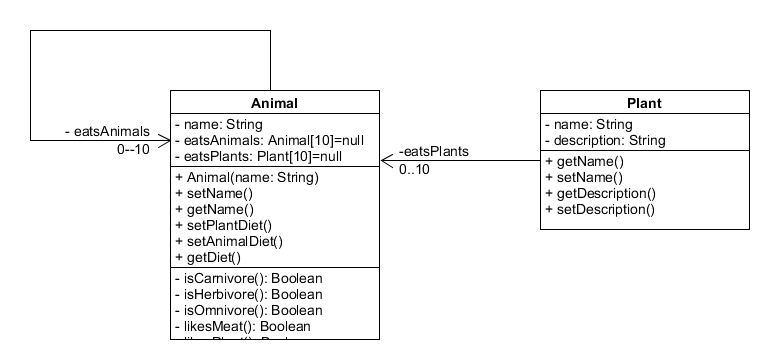
\includegraphics[width=\linewidth]{Uebung1}
\subsection*{Implementierung}
Der Code für die Klasse 'Animal' sieht aus wie folgt:
\begin{lstlisting}
public class Animal {
   //FIELDS
   private String name;
   private Animal[] eatsAnimals = new Animal[10];
   private Plant[] eatsPlants = new Plant[10];
   //CONSTRUCTOR
   public Animal(String name) {
      this.name = name;
   }
   //GETTER SETTER
   public void setName(String name) {
      this.name = name;
   }
   public String getName() {
      return name;
   }
   public void setPlantDiet(Plant plant) {
      for (int i = 0; i < eatsPlants.length; i++) {
         if (eatsPlants[i] == null) {
            eatsPlants[i] = plant;
            return;
         }
         return;
      }
   }
   public void setAnimalDiet(Animal animal) {
      for (int i = 0; i < eatsAnimals.length; i++) {
         if (eatsAnimals[i] == null) {
            eatsAnimals[i] = animal;
            return;
         }
         return;
      }
   }
   //PUBLIC METHODS
   public void getDiet() {
      if (isCarnivore()) {
         System.out.println(this.name + " is a carnivore");
      } else if (isHerbivore()) {
         System.out.println(this.name + " is a herbivore");
      } else System.out.println(this.name + " is a omnivore");
   }
   //HELPER METHODS

   private Boolean isCarnivore() {
      if (!likesPlant()) {
         return true;
      } else return false;
   
   private Boolean isHerbivore() {
      if (!likesMeat()) {
         return true;
      } else return false;
   }
   private Boolean isOmnivore() {
      if (likesMeat() && likesPlant()) {
         return true;
      } else return false;
   }
   private boolean likesMeat() {
      for (int i = 0; i < eatsAnimals.length; i++) {
         if (eatsAnimals[i] != null) {
            return true;
         }
      }
      return false;
   }
   private boolean likesPlant() {
      for (int i = 0; i < eatsPlants.length; i++) {
         if (eatsPlants[i] != null) {
            return true;
         }
      }
      return false;
   }
}
\end{lstlisting}
Der Code für die Klasse 'Plant' sieht aus wie folgt:
\begin{lstlisting}
public class Plant {
   //FIELDS
   private String name;
   private String description;
   //GETTER SETTER
   public String getName() {
      return name;
   }
   public String getDescription() {
      return description;
   }
   public void setName(String name) {
      this.name = name;
   }
   public void setDescription(String description) {
      this.description = description;
   }
}
\end{lstlisting}
Der Code für das Programm 'Biotest' sieht aus wie folgt:
\begin{lstlisting}
public class Bio_Test {
   public static void main(String[] args){
       Pflanzen_Tiere.Pflanzen Gras = new Pflanzen_Tiere.Pflanzen();
       Gras.setBeschreibung("Gras ist Gruen");

       Pflanzen_Tiere.Pflanzen Beeren = new Pflanzen_Tiere.Pflanzen();
       Beeren.setBeschreibung("Beeren sind rot");

       Pflanzen_Tiere.Tiere Zebra = new Pflanzen_Tiere.Tiere();
       Zebra.setName("Zebra");
       Zebra.setPf_futter("Gras");


       Pflanzen_Tiere.Tiere Loewen = new Pflanzen_Tiere.Tiere();
       Loewen.setName("Loewen");
       Loewen.setF_futter("Zebras");

       Pflanzen_Tiere.Tiere Baeren = new Pflanzen_Tiere.Tiere();
       Baeren.setName("Baeren");
       Baeren.setPf_futter("Beeren");
       Baeren.setF_futter("Fische");

       Zebra.ausgabe();
       Loewen.ausgabe();
       Baeren.ausgabe();
   }
}
\end{lstlisting}
Die UML-Architektur der Objektebene nach Ausführung von 'Biotest' sieht wie folgt aus:\\
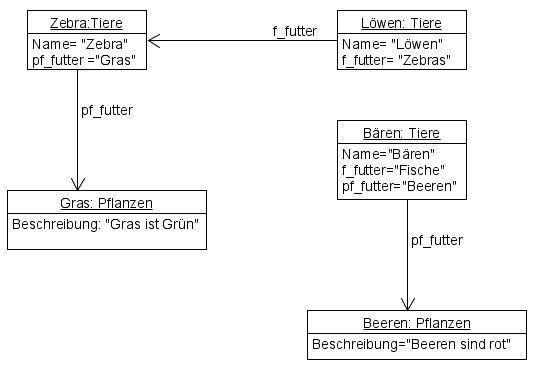
\includegraphics{objektdiagramm}


\end{document}
